\chapter{Analiză și fundamentare teoretică}
\label{ch:analysis}
\pagestyle{fancy}

\section{Protocoale de comunicatie}\label{sec:protocols}
\subsection{TCP/IP}\label{subsec:tcpip}
TCP/IP este o stiva de comunicatie, un protocol, care sta la baza internetului si a interconectivitatii dispozitivelor. Majoritatea dispozitivelor 
care suporta conexiunea la interent, de exemplu, telefoane, calculatoare personale etc, gestioneaza aceasta stiva de comunicatie. Implementeaza o arhitectura 
pe 5 nivele unde fiecare nivel poate implementa diferite protocoale specifice si este constient doar de nivelele care il inconjoara, nivelul superior 
si cel inferior lui. 

Figura \ref{fig:TCPIP_Layers} prezinta nivelele stivei de comunicatie TCP/IP in contextul a doua dispozitive conectate la un router.
\begin{figure}[H]
    \centering
    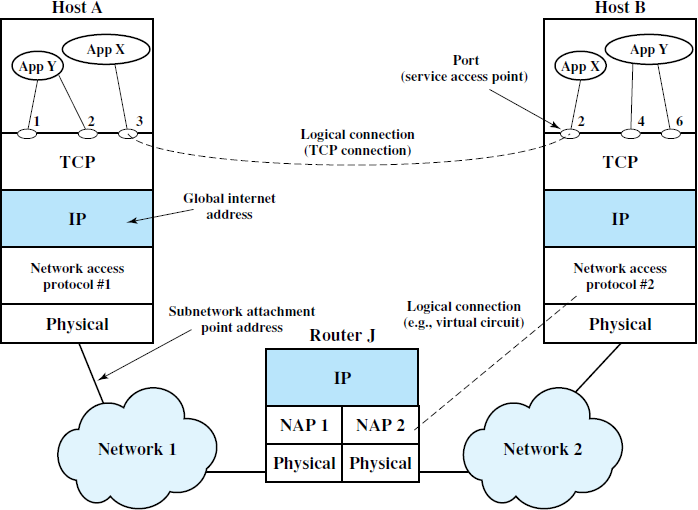
\includegraphics[scale=0.8]{figs/TCPIP_Layers.png}
    \caption{Stiva de comunicare TCP/IP \cite{williamStallings}}
    \label{fig:TCPIP_Layers}
\end{figure}

Host A si Host B reprezinta doua dispozitive conectate la un router care implementeaza stiva TCP/IP. De exemplu, un calculator personal si un telefon.

Nivelul aplicatiei, reprezentat in figura prin App X si App Y, contine protocoale de comunicatie de nivel inalt, cum ar fi protocolul HTTP, FTP, MQTT etc. 
Acest nivel trimite catre nivelul TCP informatii precum, adresa ip si portul dispozitivului destinatie.

Nivelul transport, reprezentat in figura prin TCP, Are rolul de a se asigura ca mesajele trimise de aplicatiile de la nivelul precedent ajung la destinatie 
fara erori si in ordinea in care au fost trimise. De asemenea, la acest nivel se gestioneaza si porturile aplicatiilor. 

Nivelul internet protocol, reprezentat in figura prin IP, se ocupa de transmisia datelor prin mai multe retele pana la destinatia finala. La acest nivel 
mesajului i se ataseaza adresa IP a destinatiei primita de la nivelul TCP. Astfel mesajul poate fi transmis prin mai multe retele pana atinge dispozitivul 
destinatie.

Nivelul de acces retea, reprezentat in figura prin Network access protocol \#1, se ocupa de transmisia datelor catre urmatorul dispozitiv din sub-reteaua.
lui. In cazul schemei, urmatorul dispozitiv din retea este router-ul. Nu este responsabil de destinatia finala a mesajului.

Nivelul fizic, reprezentat in figura prin Physical, se ocupa de transformarea mesajului primit de la nivelul precedent in unde radio, in cazul 
comunicatiei fara fir, sau in semnal electric sau luminos, in cazul comunicatiei pe fir si de transmisia acestuia prin retea. 

Routerul, reprezentat in figura prin Router J, implementeaza nivelele de jos ale stivei, IP, Network Access protocol, si Physical. Implementeaza doar aceste 
trei nivele din stiva, deoarece rolul lui este de a crea o legatura intre doua retele. Un mesaj primit de la un dispozitiv din reteaua 1 va fi decodat pana 
la nivelul IP, apoi recodificat cu urmatoarea destinatie si transmis.

Fiecare nivel adauga la mesajul original trimis de nivelul aplicatiei un antet si in unele cazuri si un subsol. Subsolul reprezinta un cod de verificare a 
erorilor, cum ar fi CRC, iar antetul reprezinta informatii specifice rolului nivelului de care este adaugat. La raceptia unui mesaj calea acestuia este inversa, 
de la nivelul Physical catre nivelul Application.

Termenul Socket reprezinta o pereche (Host, Port) care identifica unic un dispozitiv in tot internetul. Perechea (Host, Port) este formata din adresa globala
a unui dispozitiv si portul pe care acesta comunica. De exemplu, la crearea unei conexiuni intre doua dispozitive, initiatorul conexiunii trebuie sa cunoasca si 
sa adauge in mesajul trimis adresa globala in internet a dispozitivului destinatie si portul pe care acesta asculta. Socket-ul este utilizat la crearea unei 
conexiuni intre doua aplicatii.

\subsection{HTTP}\label{sec:http}
Protocolul de comunicatie HTTP reprezinta standardul pentru comunicarea documentelor prin internet. Acesta este utilizat cu preponderenta pentru obinerea paginilor 
web de la un server web. Este un model de comunicatie client-server, unu la unu, care defineste cum sunt formatate informatiile si trimise de catre client si 
cum trebuie sa raspuna server-ul la acestea.

Modelul de comunicatie este de tipul cerere-raspuns. Clientul trimite o adresa URL catre server, apoi asteapta un raspuns. Serverul primeste adresa, 
identifica unic un set de date, de exemplu, o pagina web sau o imagine, pe baza adresei URL, apoi returneaza un raspuns care contine informatiile cerute 
de client. Este un protocol de comunicatie sincron, deoarece se asteapta raspunsul la crerere, spre deosebire de alte protocoale de comunicatie, 
de exemplu, MQTT, unde se trimit date catre server fara a se astepta un raspuns la acestea.

HTTP este utilizat pentru tranzactionarile de date mari, neavand o limita superioara de dimensiune a pachetului. Totusi dimensiunile utilizate in mod 
uzual sun relativ mici din cauza timpului de raspuns care creste odata cu dimensiunea resursei.

In stiva de comunicare a protocolului TCP/IP, HTTP se afla in nivelul cel mai inatlt, si anume, nivelul aplicatiei. Acest lucru inseamna ca HTTP nu se 
ocupa de transportul efectiv al mesajelor printr-o retea, ci doar defineste un limbaj comun pentru arhitectura de comunicatie client-server.  

Antetul unui mesaj este bazat pe text, insemnand ca particularitatile mesajelor sunt reprezentate prin cuvinte intuitive spre deosebire de MQTT unde 
particularitatile sunt reprezentate prin biti sau set de biti. Mai jos sunt prezentate cele mai uzuale astfel de proprietati:
\begin{itemize}
	\item Content-Type - specifica in ce format sunt codate datele cuprinse in corpul mesajului. Valoarea acestuia poate fi JSON, XML etc.
	\item Content-Length - specifica dimensiunea corpului mesajului. Cum s-a precizat si mai sus, nu exista o valoare maxima petru acest camp, dar 
	in mod uzual nu depaseste 256MB.
    \item Accept - formate ale datelor care sunt acceptate de catre client ca raspuns. De exemplu, un client poate cere unui server un set de imagini si 
    prin acest camp informeaza server-ul sa-i ofere doar imagini in format jpeg.
    \item User-Agent - utilizat de client pentru a specifica informtii despre el insusi, de exemplu, tipul aplicatiei, versiunea etc.
    \item Connection - poate lua doua valori, "keep-alive" si "close". Este utilizat de client pentru a specifica daca doreste sa fie incheiata conexiunea 
    dupa returnarea raspunsului. "keep-alive" va informa serverul ca actuala conexiune va ramane deschisa pentru un nou request, iar "close" il va 
    informa ca va fi incheata conexiunea.
\end{itemize}

\

O metoda HTTP reprezinta o actiune pe care un client o trimite unui server pentru a fi executata. Cele mai comune metode HTTP sunt:
\begin{itemize}
	\item GET - prin aceasta metoda clientul cere o resursa server-ului
	\item POST - prin aceasta metoda clientul trimite un set de date catre server pentru a modifica o resursa sau pentru a salva o resursa noua. Daca 
	adresa URL contine o resursa care nu exista deja, cererea va returna codul de eroare 404.
	\item PUT -  prin aceasta metoda clientul trimite un set de date catre server pentru a suprascrie o resursa sau pentru a crea o resursa noua. Daca 
    este trimis un URL cu o resursa care nu exista, aceasta va fi creata.
	\item DELETE - prin aceasta metoda clientul sterge o resursa de pe server.
\end{itemize}

\

O adresa URL este compusa din trei parti principale:
\begin{itemize}
	\item Protocolul utilizat pentru extragerea resursei. In general acesta este HTTP si este de forma "http://".
	\item Adresa serverului sau locatia serverului. De exempu, www.universitatea\_tehnica.ro.
	\item Identificatorul unic al resursei. De exemplu, /clientID/1 sau /index.html.
\end{itemize}

\

Codul de status este un cod returnat de server in raspuns care instiinteaza clientul de statusul executiei cererii. Sunt foarte multe coduri de eroare 
impartite pe categorii de erori, fiecare reprezentand o eroare diferita. Mai jos sunt enumerate cele mai utilizate coduri de eroare:
\begin{itemize}
	\item 200 - Success. Serverul instiinteaza clientul ca actiunea a fost executata cu success.
	\item 400 - Bad Request. Serverul nu accepta cererea clientului, deoarece aceasta este eronata. 
	\item 403 - Forbidden. Este trimisa de server atunci cand clientul nu are autoritatea sa acceseze o anumita resursa.
	\item 404 - Not found. Resursa ceruta de client nu poate fi gasita. 
\end{itemize}

\

\subsection{MQTT}\label{sec:mqtt}
Standardul MQTT defineste un set de reguli, un limbaj, pe care doua sau mai multe entitati trebuie sa il respecte pentru a putea schimba mesaje intre 
ele. Entitatile acestuia sunt clientii si un server, numit Broker. Este un protocol pentru transmiterea mesajelor prin internet care necesita resurse reduse si 
utilizeaza un model de comunicatie de tip publica/aboneaza. In mod uzual opereaza impreuna cu stiva de comunicatie TCP/IP, dar poate fi integrat si cu alte 
standarde, cum ar fi ZigBee sau LoRa. Acest protocol este foarte utilizat in domeniul Internetul Lucrurilor fiind potrivit pentru 
senzorii cu capacitati de procesare reduse si oferind un grad inalt de scalabilitate prin structura de functionare a acestuia. In urmatoarele paragrafe 
din acest capitol vom analiza caracteristicile cheie ale acestui protocol.

Broker-ul este un server, o unitate centrala, specializat pe receptia mesajelor de la clienti si retransmisia acestora catre clientii interesati de 
tipul de mesaj respectiv. Acesta poate fi vizualizat ca o unitate de decuplare, deoarece clientii nu comunica direct intre ei, ci prin acest manager de 
mesaje. Comunicarea este de tip asincrona, calea unei tranzactii porneste de la client si se opreste la Broker, deci o tranzactie nu implica doi clienti 
in acelasi timp. 

Modelul de comunicatie publica/aboneaza imparte clientii in doua categorii, clienti care publica, transmit, mesaje catre Broker si clienti care se aboneaza
la Broker pentru a receptiona mesajele publicate. Clientii pot avea ambele roluri, si de publicatori si de abonati, pastrand rolurile disjuncte. Astfel ca 
un client care are ambele roluri va publica periodic un set de date si in acelasi timp va fi abonat la Broker pentru receptia de mesaje de la unul sau mai 
multi clienti. In mod uzual aceste roluri pot fi impartite in doua categorii, rol principal si rol secundar. In cazul uni senzor, rolul principal este 
de a publica date despre mediul inconjurator, iar rolul secundar este de abonare pentru a receptiona modificari ale configuratiilor acestuia, de exemplu, 
perioada la care se face publicarea. In cazul unui client smartphone sau pagina web, rolul principal este de abonat pentru a receptiona metricile de la senzori, 
iar rolul secundar este de publicator pentru transmisia de configuratii catre senzor.

Figura \ref{fig:MQTTBrokerArchitecture} prezinta arhitectura publica/aboneaza a protocolului de comunicatie MQTT. Fiecare modul prezentat in figura este 
descris in paragrafele de mai sus.
\begin{figure}[H]
    \centering
    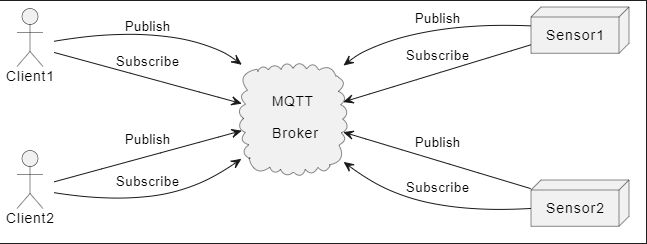
\includegraphics[scale=0.8]{figs/MQTTBrokerArchitecture.png}
    \caption{Arhitectura publica/aboneaza a protocolului MQTT}
    \label{fig:MQTTBrokerArchitecture}
\end{figure}

Subeictul mesajelor, denumit topic in standard \cite{mqttstandard}, reprezinta o serie de cuvinte structurate pe nivele care descriu intr-un mod succint datele mesajului. 
Aceste cuvinte sunt separate prin caracterul special "/", denumit si separator de nivel, si au rolul de a filtra mesajele trimise catre clienti. 
De exemplu, Un senzor transmite un mesaj care contine date de temperatura catre Broker sub subiectul "IDsenzor/citiri/temperatura". 
Broker-ul va redirectiona acest mesaj doar catre clientii care sunt abonati pentru receptia de mesaje care au subiectul "IDsenzor/citiri/temperatura".

Structura unui mesaj MQTT este de tip binar, fiecare bit sau grupare de biti indentifica un tip de mesaj sau diferite proprietati, in comparatie cu alte 
protocoale de comunicatie care utilizeaza un format bazat pe text, unde tipurile de mesaje sau proprietatile sunt identificate prin text, de exemplu,
protocolul de comunicatie HTTP. Principalul avantaj al formatului de tip binar este dimensiunea scazuta a pachetului. Tabelul \ref{tab:StructuraMesajMQTT} 
contine o prezentare generala a acestui pachet unde:
\begin{itemize}
	\item Control Field - reprezinta octetul de control al pachetului si este impartit in doua zone:
    \begin{itemize}
        \item Tipul pachetului in primii 4 biti
        \item Semnale pentru activarea sau dezactivarea unor proprietati
    \end{itemize}
	\item Remaining Length - poate avea o lungime cuprinsa intre 1 si 4 octeti si reprezinta lungimea ramasa in pachet, adica lungimea campurilor Variable Header 
    si Payload
	\item Variable Header - are o lungime variabila care este cuprinsa in campul precedent. Acest camp difera in functie de tipul mesajului, de exemplu, in 
	cazul mesajului de publicare a datelor acest camp contine subiectul.
	\item Payload - are o lungime variabila care este cuprinsa in campul Remaining Length si reprezinta partea utila a mesajului, de exemplu, datele citite de 
	la senzor.
\end{itemize}

\begin{table}[ht]
    \caption{Structura mesaj MQTT}
    \centering                          % tabel centrat
    \begin{tabular}{|c|c|c|c|}          % 4 coloane centrate
        \hline
        1 B & 1-4 B & x B & x B \\ [0.5ex]   % inserare tabel
        %heading
        \hline                              % linie orizontal simpla
        Control Field & Remaining Length & Variable Header & Payload \\               % corpul tabelului
        \hline
    \end{tabular}
    % titlul tabelului
    \label{tab:StructuraMesajMQTT}                % eticheta folosita pentru referirea tabelului in text; referirea in text se va face cu \ref{table:nonlin}
\end{table}

Tranzactia reprezinta un schimb de mesaje intre un client si Broker si are o structura de tip cerere si confirmare. Cererea este un mesaj care contine informatii 
utile, de exemplu, datele unui senzor sau datele necesare conectarii la Broker, iar confirmarea este un mesaj prin care Borker-ul instiinteaza clientul ca cererea 
lui a fost inregistrata. Acestea din urma sunt transmise si in caz de eroare si in caz de success, iar acest lucru este semnalat in campul "Variable Header" 
prezentat in tabelul \ref{tab:StructuraMesajMQTT}. Protocolul MQTT contine mai multe tipuri de mesaje impartite pe cele doua categorii prezentate mai sus dintre 
care cele mai importante sunt prezentate in cele ce urmeaza:
\begin{itemize}
    \item CONNECT - acest pachet este trimis de catre client pentru a realiza o conexiune cu Broker-ul.
    \item CONNACK - acest pachet este trimis de catre Broker si reprezinta raspunsul pentru mesajul CONNECT si are rolul de a confirma realizarea conexiunii.
    \item PUBLISH - acest pachet este trimis de catre client si contine subiectul si datele utile.
    \item PUBACK - acest pachet este trimis de catre Broker ca raspuns la mesajul PUBLISH.
    \item SUBSCRIBE - acest pachet este trimis de catre client si reprezinta cererea de abonare la un anumit subiect. Subiectul este continut in pachet.
    \item SUBACK - acest pachet este trimis de catre Broker si reprezinta confirmarea subscriptiei clientului.
\end{itemize}

Conexiunea dintre client si Broker se realizeaza la cererea clientului print trimiterea unui mesaj specific. Acest tip de mesaj contine un camp special 
denumit "keep alive" prin care clientul informeaza Broker-ul de durata de viata a conexiunii dintre acestia. Clientul poate alege inchiderea conexiunii 
cu Broker-ul dupa fiecare mesaj de publicare a datelor cu scopul de a intra intr-un mod de consum de putere redus pana la urmatoarea perioada de 
publicare. Salvarea energiei aduce cu sine cresterea numarului de mesaje interschimbate intre client si Broker, dar aduce avantaje in durata de viata 
a bateriei. 

\subsection{Wi-Fi}\label{sec:wifi}
Wi-Fi reprezinta un set de protocoale de comunicatie fara fir bazate pe standardul IEEE 802.11. In stiva TCP/IP acesta este implementat in ultimele 2 nivele, 
Network Addressing (MAC) si Physical. Acesta permite crearea unei retele locale de dispozitive interconectate fara cabluri fizice.

O retea Wi-Fi uzuala este formata din doua tipuri de dispozitive, statii de baza si statii client. Statiile de baza reprezinta punctul central al unei retele Wi-Fi 
si gestioneaza conexiunea si distribuirea mesajelor intre statiile client connectate la aceasta. Statiile client nu pot comunica direct intre ele, ci prin 
intermediul statiei de baza. Acest tip de retea este utilizat cu preponderenta pentru a oferi statiilor client conexiune la internet. Pentru acest lucru 
statia de baza este connectata la un modem care la randul lui este conectat la reteaua furnizorului de internet.

Un alt tip de retea Wi-Fi, mai putin utilizata, este reteaua punct la punct si este formata doar din statii client interconectate intre ele in mod direct. 
Acest tip de retea utilizeaza un protocol numit Wi-Fi Direct si este utilizata pentru conexiuni si tranzactii de date intre doua statii client.

Nivelul Physical are rolul de a codifica si decodifica semnalele digitale in semnale radio in benzile de frecventa 2.4GHz si 5GHz. Aceste benzi fac parte din 
din benzile de frecventa ISM alocate pentru utilizarea in domeniile industrial, stiintific si medical. Petru codificarea si decodificarea datelor 
sunt utilizate mai multe scheme de modulatie, din care, schema de modulatie OFDM este utilizata cu preponderenta. 

Banda de frecventa 2.4GHz reprezinta intervarul de frecvente cuprins intre 2.4GHz si 2.5GHz. Acest interval de 100 MHz este impartit in 14 canale partial 
suprapuse. Fiecare canal are o latime de banda de 22 MHz. Majoritatea dispozitivelor ofera utilizatorului posibilitatea de a schimba canalul de comunicatie 
cu scopul imbunatatirii vitezei. O viteza mai buna este obtinuta prin scaderea interferentei dintre dispozitivele dintr-o retea, acest lucru fiind obtinut 
prin imprastierea dispozitivelor pe cele 14 canale. 

Figura \ref{fig:2400MHz_channels} prezinta modul in care banda de frecventa 2.4GHz este impartita in cele 14 canale. Fiecare canal are notat deasupra lui 
numarul si centrul frecventei acestuia.
\begin{figure}[H]
    \centering
    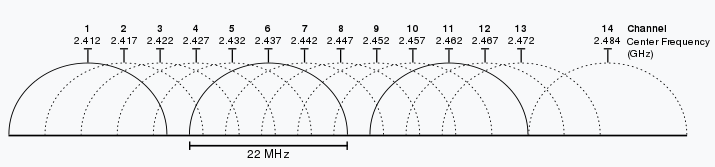
\includegraphics[scale=0.8]{figs/2400MHz_channels.png}
    \caption{Canalele de comunicatie in banda de frecventa 2.4GHz \cite{wifichannels}}
    \label{fig:2400MHz_channels}
\end{figure}

Nivelul MAC are rolul de a gestiona si mentine comunicatia intre o statie client si o statie de baza dintr-o retea locala. Acesta este responsabil de 
transmiterea pachetului de la statia client catre statia de baza, de retransmiterea pachetului in cazul in care acesta nu a fost receptionat de catre 
statia de baza, de evitare a coliziunilor cu alte dispozitive din retea etc.

Conexiunea dintre o statie client si o statie de baza se poate realiza in doua moduri, activ sau pasiv. In modul activ, statia client transmite pachete 
care contin informatii despre capabilitatile lui, iar statiile de baza raspund la aceste pachete cu numele retelei si alte informatii legate de retea. 
In modul pasiv, statia de baza transmite periodic pachete prin care isi anunta prezenta, iar statiile client intra in receptie pe fiecare canal cu scopul 
de a receptiona un astfel de frame. Dupa acest prim pas, urmeaza un schimb de pachete prin care se realizeaza conexiunea dintre statia client si statia de baza.

Acest protocol, in comparatie cu un protocol pe fir, faciliteaza instalarea unei retele locale prin inlaturarea necesitatii cablurilor si a rutarii acestora 
si mobilitatea dispozitivelor din retea fiind permisa deplasarea dispozitivelor in raza de acoperire a statiei de baza. De asemenea, principalele dezavantaje 
ale acestuia sunt interferenta dintre dispozitivele din retea si raza de acoperire a statiei de baza.

\subsection{SPI}\label{sec:spi}
SPI, Serial Peripheral Interface, este un protocol de comunicatie seriala si sincrona. Arhitectura acestuia este formata din dispozitive care pot avea 2 
roluri, master sau slave. Intr-o arhitectura SPI poate exista un singur dispozitiv master si unul sau mai multe dispozitive slave. Acest protocol a fost 
proiectat pentru communicatia dintre un microcontroller, dispozitivul master, si perifericele acestuia, dispozitivele slave. 

Liniile de semnal utilizate in protocolul SPI sunt:
\begin{itemize}
    \item SS (Slave Select) este un semnal controlat de dispozitivul master prin care activeaza dispozitivul slave pentru o transmisie de date.
    \item SCLK (Serial Clock) este un semnal generat de dispozitivul master pentru sincronizarea cu dispozitivul slave in timpul unei transmisii de date.
    \item MOSI (Master Out Slave In) este semnalul de date prin care dispozitivul master transmite date dispozitivului slave. Aceasta linie de semnal 
    poate sa lipseasca in anumite moduri de comunicatie.
    \item MISO (Master In Salve Out) este semnalul de date prin care dispozitivul slave transmite date dispozitivului master. Aceasta linie de semnal 
    poate sa lipseasca in anumite moduri de comunicatie.
\end{itemize}

\

Comunucatia dintre doua dispozitive, master si slave, se poate realizeaza prin 3 sau 4 linii de semnal. Modul de communicatie cu 3 linii de semnal se poate 
numi Simplex sau Half-Duplex, iar cel cu 4 linii de semnal Full-Duplex:
\begin{itemize}
    \item Simplex reprezinta modul de comunicatie in care doar dispozitivul master poate transmite date catre unul sau mai multe dispozitive slave. Liniile 
    de semnal utilizate sunt SS, SCLK si MOSI.
    \item Half-Duplex reprezinta modul de comunicatie in care este utilizata o singura linie de date, comuna intre un dispozitiv master si unul sau mai multe 
    dispozitive slave, pentru transmisia de date de la master catre slave sau de la slave catre master. Un singur dispozitiv poate transmite la un moment dat. 
    Liniile de semnal utilizate sunt SS, SCLK si MOSI/MISO.
    \item Full-Duplex reprezinta modul de comunicatie cel mai utilizat. Acesta utilizeaza 2 linii de date pentru tranzactionarea intre un dispozitiv master 
    si unul sau mai multe dispozitive slave. O linie este utilizata pentru transmisia de date de la master catre slave si una pentru transmisia datelor de 
    la slave catre master. Dispozitivela master si slave pot transmite date simultan. Liniile de semnal utilizate sunt SS, SCLK, MOSI si MISO.    
\end{itemize}

Figura \ref{fig:SPIMasterSlave} prezinta modul de comunicatie Full-Duplex al protocolului SPI dintre un dispozitiv master si doua dispozitive Slave.
\begin{figure}[H]
    \centering
    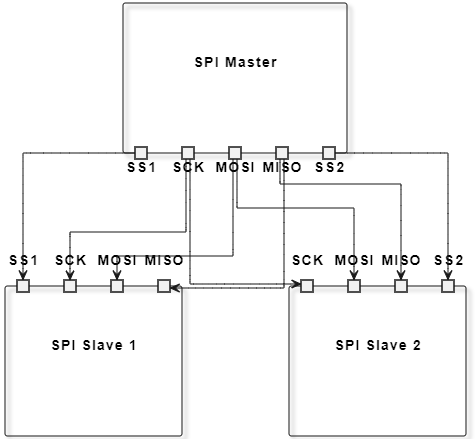
\includegraphics[scale=0.8]{figs/SPIMasterSlave.png}
    \caption{Arhitectura protocolului SPI Full-Duplex}
    \label{fig:SPIMasterSlave}
\end{figure}

Intr-o arhitectura SPI in care exista mai multe dispozitive slave, dispozitivul master are o line de semnal SS specifica fiecarui dispozitiv slave, iar liniile 
de semnal SCK, MOSI si MISO sunt comune. Astfel, atunci cand dispozitivul master initiaza o tranzactie cu un dispozitiv slave, activeaza linia de semnal SS 
legata la acel slave, celelalte dispozitive slave ramanand inactive.

Un alt mod, mai putin utilizat, in care liniile de semnal pot fi legate intre un dispozitiv master si mai multe dispozitive slave este prin inlantuirea 
dispozitivelor slave. Astfel, dispozitivul master are o singura linie de semnal SS comuna pentru toate dispozitivele slave, linia de semnal MOSI este legata 
la primul dispozitiv slave din lant, iar linia MISO este legta la ultimul dispozitiv slave din lant. La initierea unei tranzactii, dispozitivul master activeaza 
toate dispozitivele slave, transmite date catre primul dispozitiv slave din lant, iar fiecare slave din lant redirectioneaza datele catre urmatorul. Atunci cand 
datele transmise de master ajung la dispozitivul slave cu care se doreste comunicarea, acesta proceseaza datele si redirectioneaza un mesaj nou catre urmatorul 
slave. Acest mod de comunicare este utilizat doar in cazul in care nu este posibila rutarea unui semnal SS catre fiecare dispozitiv slave.

Protocolul SPI permite gestionarea polaritatii si a fazei semnalului de ceas pentru prelevarea datelor. Dispozitivul master este responsabil de utilizarea 
polaritatii si a fazei suportate de dispozitivul slave. Tabelul \ref{tab:spiPolPhase} prezinta cele 4 moduri in care datele pot fi prelevate.
\begin{table}[ht]
    \caption{Polaritateaa si faza semnalului de ceas}
    \centering   % tabel centrat
    \renewcommand{\arraystretch}{2.2}
    \begin{tabular}{|c|c|c|}          % 4 coloane centrate
        \hline
        Polaritate & Faza & Descriere \\ [0.5ex]   % inserare tabel
        %heading
        \hline                          % linie orizontal simpla
        0 & 0 & \parbox{280pt}{SCLK are valoarea 0 logic cand este inactiva, iar datele sunt prelevate pe frontul crescator}\\ 
        0 & 1 & \parbox{280pt}{SCLK are valoarea 0 logic cand este inactiva, iar datele sunt prelevate pe frontul descrescator}\\ 
        1 & 0 & \parbox{280pt}{SCLK are valoarea 1 logic cand este inactiva, iar datele sunt prelevate pe frontul descrescator}\\ 
        1 & 1 & \parbox{280pt}{SCLK are valoarea 1 logic cand este inactiva, iar datele sunt prelevate pe frontul crescator}\\ 
        \hline
    \end{tabular}
    % titlul tabelului
    \label{tab:spiPolPhase}                % eticheta folosita pentru referirea tabelului in text; referirea in text se va face cu \ref{table:nonlin}
\end{table}

Figura \ref{fig:SPITimingDiagram} prezinta in detaliu modul in care sunt tranzactionate date intre un dispozitiv master si unul slave. Este prezentat modul de 
comunicatie Full-Duplex cu semnalul de ceas avand caracteristicile de polaritate si faza 0 si 0, adica semnalul SCLK are valoare 0 in modul inactiv, iar datele 
sunt prelevate pe frontul crescator.
\begin{figure}[H]
    \centering
    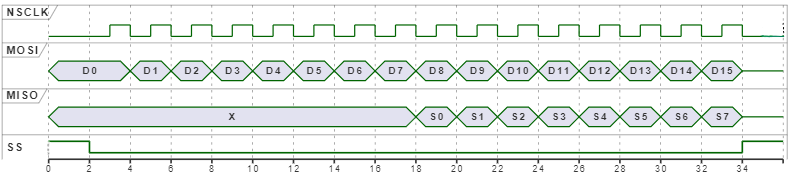
\includegraphics[scale=0.75]{figs/SPITimingDiagram.png}
    \caption{Diagrama de timp a comunicatiei SPI}
    \label{fig:SPITimingDiagram}
\end{figure}

Datele sunt transmise intre un dispozitiv master si unul slave bit cu bit. Dispozitivul master activeaza linia SS prin tranzitia din 1 logic in 0 logic, 
apoi seteaza linia MOSI in conformitate cu primul bit din secventa de biti care urmeaza a fi tranzactionata si genereaza semnalul de ceas. Dupa ce ultimul 
bit a fost transmis, dispozitivul master mentine semnalul de ceas in 1 logic sau in 0 logic in functie de setarea polaritatii, iar apoi dezactiveaza linia 
SS prin tranzitia din 0 logic in 1 logic. De exemplu, in cazul in care semnalul de ceas are caracteristicile de polaritate si faza 0 si 0, pe frontul 
crescator al semnalului de ceas dispozitivul slave citeste starea liniei de semnal MOSI, 1 logic sau 0 logic, iar pe frontul descrescator dispozitivul master 
schimba sau mentine starea liniei conform cu urmatorul bit care urmeaza a fi transmis. In acelasi timp, dispozitivul slave poate tranzitiona linia de date MISO 
in conformitate cu secventa de biti pe care acesta doreste sa o trimita dispozitivului master.

Viteaza de transmisie a acestui protocol este foarte mare in comparatie cu alte protocoale de comunicatie asemanatoare, cum ar fi I2C. Nu ofera un mechanism 
de verificare a erorilor sau de instiintare ca datele au fost receptionate cu success de cealalta parte. Aceste doua dezavantaje pot fi intampinate prin 
utilizarea unui algoritm de verificare a integritatii datelor si a unui mecanism de tip cerere raspuns.

\subsection{I2C}\label{sec:i2c}
I2C este un protocol de comunicatie seriala creat pentru comunicatia dintre un microcontroler si unul sau mai multe periferice ale acestuia. Este un 
protocol sincron, are o arhitectura de tip master slave si necesita doar doua linii de semnal pentru tranzactionarea de date. 

Acest protocol identifica fiecare dispozitiv conectat la magistrala printr-o adresa unica, spre deosebire de alte protocoale precum SPI care necesita cate o 
linie de semnal pentru fiecare dispozitiv sau o inlantuire a dispozitivelor. De asemenea, utilizeaza doar 2 linii de semnal indiferent de numarul de dispozitive 
conectate la magistrala.

Liniile de semnal utilizate sunt numite SDA si SCL, linia de date si respectiv linia de ceas. Acestea sunt bidirectionale, insemnand ca ambele dispozitive 
care participa intr-o tranzactie au control asupra lor. Semnalul de ceas este generat de dispozitivul master, dar dispozitivul slave are capacitatea de a 
forta linia in stare inactiva in cazul in care nu este pregatit pentru a receptiona sau transmite date. De exemplu, dispozitivul slave nu a terminat de 
procesat o sarcina si forteaza linia de ceas in stare inactiva pentru a anunta dispozitivul master sa nu trimita urmatoarele date. Cand sarcina este finalizata, 
dispozitivul slave elibereaza linia de ceas, iar tranzactia datelor isi reia cursul.

Ofera capabilitatea mai multor dispozitive master conectate la aceeasi magistrala. Doar un dispozitiv master poate controla magistrala la un moment dat. 
Decizia de control este luata prin verificarea liniilor magistralei, daca acestea sunt inactive, au valoarea 1 logic, magistrala este libera pentru un transfer,
iar daca acestea sunt ocupate inseamna ca exista o tranzactie in curs de procesare initiata de un alt dispozitiv master de pe magistrala. Pentru a detecta 
corect daca magistrala este libera sau nu, verificarea liniilor trebuie efectuata pentru cel putin o perioada de ceas, deoarece liniile SCL si SDA pot avea 
valoarea 1 logic simultan pentru o jumatate din perioada de ceas.

Figura \ref{fig:I2CBus} prezinta un exemplu de magistrala I2C cu 6 dispozitive conectate. Microcontroller A si Microcontroller B reprezinta dispozitivele master, 
iar celelalte reprezinta dispozitive slave, ecran LCD, convertor din semnal analogic in semnal digital etc.
\begin{figure}[H]
    \centering
    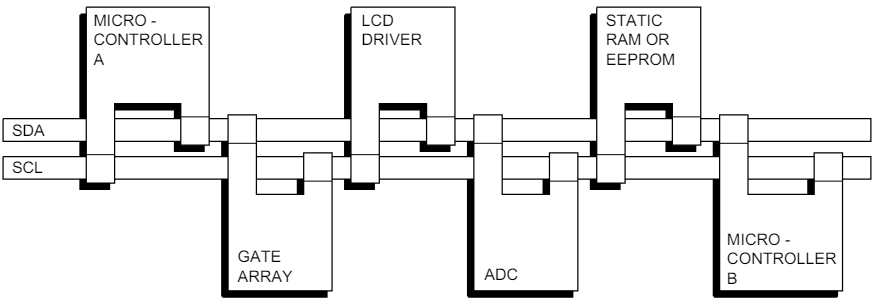
\includegraphics[scale=0.68]{figs/I2CBus.png}
    \caption{Exemplu de magistrala I2C \cite{i2ctutorial}}
    \label{fig:I2CBus}
\end{figure}

Un transfer de date pe magistrala I2C este efectuat in mai multe etape, prima etapa dupa verificarea disponibilitatii magistralei este transmisia unei conditii 
de start. Aceasta conditie este reprezentata de tranzitia din 1 logic in 0 logic a liniei SDA in timp ce linia SCL este in 1 logic si informeaza dispozitivele 
legate la magistrala ca o noua tranzactie este initiata.

A doua etapa este reprezentata de transmisia primului octet care contine adresa dispozitivului slave cu care se va efectua transferul de date pe primii 7 biti si 
a bitului care indica o citire sau o scriere. Toate dispozitivele conectate la magistrala I2C vor receptiona acest octet si il vor compara cu adresa proprie. 
Dispozitivul care este identificat de adresa transmisa va confirma receptia acesteia.

Fiecare octet transmis de un dispozitiv este confirmat sau negat de catre dispozitivul care l-a receptionat. Dispozitivul master ofera un al 9-lea semnal de ceas 
dispozitivului receptor pentru aceasta confirmare. In cazul receptionarii cu success, dispozitivul receptor va mentine linia de date SDA in 0 logic pentru cea de-a 
9-a perioada de ceas (ACK), iar in cazul receptionarii eronate, acesta va mentine linia in 1 logic (NACK).

A treia etapa este reprezentata de transmisia datelor octet cu octet. In cazul unei citiri, dispozitivul master va genera semnalul de ceas, iar dispozitivul slave 
va pune primul octet de date pe linia SDA, urmand apoi al 9-lea puls de ceas prin care dispozitivul master va confirma receptia. In cazul unei scrieri, dispozitivul 
master va genera semnalul de ceas si va pune primul octet de date pe linia SDA, iar dispozitivul slave va confirma receptia acestora.

A patra etapa este transmisia conditiei de stop. Aceasta conditie este reprezentata prin tranzitia liniei de date din o logic in 1 logic  in timp ce linia 
de ceas este in 1 logic. Aceasta conditie reprezinta finalul unei tranzactii intre un dispozitiv master si unul slave.

Pentru cresterea numarului de dispozitive care pot fi conectate la o magistrala si pentru a evita coliziunea de adrese, protocolul I2C ofera capabilitatea 
de a utiliza adrese pe 10 biti. Acest lucru inseamna ca adresarea se va face in primii doi octeti transmisi de dispozitivul master pe magistrala. Primul octet 
contine biti de identificare a tipului de adresare si partea mai semnificativa din adresa, iar al doilea octet contine partea mai putin semnificativa a adresei.

Figura \ref{fig:I2CCompleteDataTransfer} prezinta etapele unei tranzactionari de date intre un dispozitiv master si unul slave.
\begin{figure}[H]
    \centering
    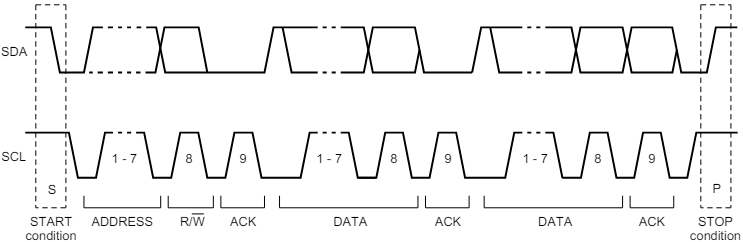
\includegraphics[scale=0.75]{figs/I2CCompleteDataTransfer.png}
    \caption{Exemplu de tranzactie I2C intre un dispozitiv master si unul slave \cite{i2ctutorial}}
    \label{fig:I2CCompleteDataTransfer}
\end{figure}

Pe durata unei transmisii, dispozitivul master sau cel slave poate in orice moment, chiar si in mijlocul transferului unui octet, sa forteze linia de ceas SCL in 
0 logic pentru a opri temporar tranzactia de date. Un exemplu de moment in care un dispozitiv efectueaza aceasta operatie este cand in mijlocul unui transfer 
de date acesta este intrerupt de o rutina interna sau de un alt periferic cu prioritate mai mare. In acest caz linia de ceas SCL va fi mentinuta in 0 logic pana 
la finalizarea executiei rutinei mai prioritare, iar apoi executia transferului I2C va fi reluat. 

Dezavantajele acestui protocol sunt viteza de maximum 3 MHz, mai mica decat cea a protocolulul SPI, si ofera doar modul Half-Duplex, un singur dispozitiv master 
sau slave poate transmite sau receptiona la un moment dat. Are ca avataje capabilitatea de conectare a mai multor dispozitive la magistrala fara a creste numarul 
de linii de semnal, bitul de confirmare al receptiei fiecarui pachet si capabilitatea de a avea mai multe dispozitive master conectate la aceeasi magistrala.

\section{Modele abstracte}\label{sec:modele}
\subsection{RESTful API}\label{sec:restapi}
RESTful semnifica Representational State Transfer Application Programmin Interface si reprezinta un set de reguli care trebuie respectate in construirea 
unei arhitecturi web pentru a beneficia de cerinte non-functionale precum, un grad mare de scalabilitate, reliabilitate si adaptabilitate. Acest set de 
reguli are ca scop decuplarea in grad cat mai mare a clientului de sarcinile serverului. In paragrafele urmatoare se vor detalia caracteristicile cheie 
ale stilului arhitectural RESTful.

API semnifica Application Programming Interface si reprezinta o interfata intre client si server in care atributiile serverului sunt de a oferi 
clientului servicii prin care acesta poate obtine si stoca date intr-o baza de date. Alte functionalitati care se doresc a fi implementate trebuie 
sa fie in sarcina clientului, deci clientul trebuie sa se asigure ca cererea pe care o trimite catre server contine toate informatiile necesare. 
De exemplu, serverul nu retine informatii de securitate, ci aceste informatii trebuie continute in pachetul trimis de catre cient.

Figura \ref{fig:RESTfulStructure} prezinta structura unei arhitecturi RESTful. Fiecare modul va fi descris in paragrafele urmatoare.
\begin{figure}[H]
    \centering
    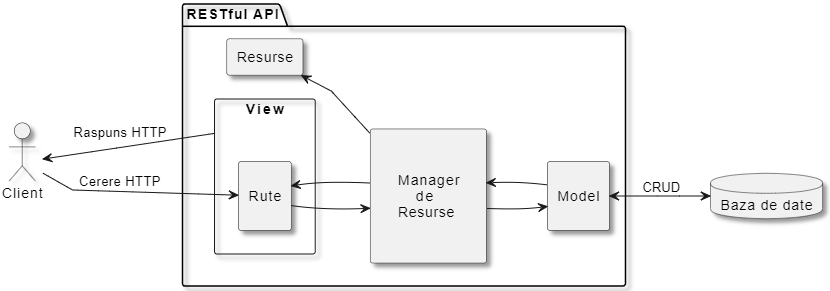
\includegraphics[scale=0.7]{figs/RESTfulStructure.png}
    \caption{Structura arhitecturii RESTful}
    \label{fig:RESTfulStructure}
\end{figure}

Principalul modul din arhitectura RESTful este modulul Resources, care semnifica resursa. O resursa reprezinta un set de date pe care un client il poate 
cere serverului prin transmiterea unui URL. Detalii despre URL se gasesc in capitolul \ref{sec:http}. Acesta reprezinta un identificator unic pentru 
fiecare resursa. Nu este necesar ca o resursa sa implementeze toate metodele HTTP, daca o metoda nu este implementata va fi returnat raspunsul de eroare 
405 semificand ca metoda nu este permisa. Exemplu de tranzactie intre client si server cu accentul pe resurse:
\begin{enumerate}
	\item clientul trimite un URL catre server
	\item serverul identifica resursa asociata URL-ului
	\item serverul interogheaza baza de date pentru resursa specificata
	\item serverul trimite un raspun care contine resursa ceruta si un status al tranzactiei
\end{enumerate}

Modulul Routes se ocupa de partea de rutare a cererilor primite de la client. Acest modul identifica pe baza adresei URL resursa de care clientul are nevoie, 
iar apoi informeaza modulul Resource Manager in legatura cu aceasta resursa.

Modulul Model se ocupa de operatiile cu baza de date, operatiile CRUD. Aceste operatii sunt creare, citire, modificare si stergere a unei intrari din 
baza de date. Rezultatul operatiei cu baza de date este returnat modulului Resource Manager.

Modulul Resource Manager este modulul central al acestei structuri si se ocupa cu extragerea resursei primita de la modulul Routes si a metodelor specifice 
acesteia, de exemplu, metodele HTTP GET si POST. Bazat pe aceste metode, modulul Resource Manager interogheaza baza de date. Raspunsul primit de la baza de date 
este validat si trimis catre modulul View.

Modulul View are sarcina de a formata datele primite de la modulul Resource Maganer in structura la care clientul se asteapta, apoi trimitand raspunsul catre 
client. 

Arhitectura RESTful API este asemanatoare cu modelul de design MVC, care semnifica Model View Controller si reprezinta o structurare a software-ului intern 
in trei module separate, Model si View care sunt identice cu modelele Model si View din RESTful API si Controller care inlocuieste modulul resource Manager 
din RESTful API.

Setul de reguli ce trebuie respectate pentru implementarea unei arhitecturi RESTful cuprind:
\begin{enumerate}
	\item Arhitectura aplicatiei trebuie sa fie de tipul client-server. Clientul trebuie separat de srever si de operatiile cu baza de date. Fiecare 
    participant al unei tranzactii trebuie sa fie independent de ceilalti.
	\item Lipsa starii inseamna ca o cerere trimisa de client trebuie sa contina toate informatiile necesare pentu ca aceasta sa fie onorata. Serverul 
	nu are voie sa retina informatii legate de client.
    \item Interfata uniforma specifica ca structura adreselor URL trebuie sa fie definita foarte clar, deoarece acestea reprezinta identificatorii unici 
    ai resurselor si implicit indentificarea corecta a resursei dorite.
    \item Clientul sau o alta componenta din retea poate sa retina raspunsurile de la server care sunt semnalate ca fiind memorabile cu scopul 
    optimizarii. 
    \item System pe nivele inseamna ca fiecare nivel este constient doar de nivelele din imediata apropiere a lui si ca intre server si client mai pot fi 
    adaugate nivele precum un server proxy.
\end{enumerate}

O metoda de versionare a software-ului unui server este prin adaugarea in adresa URL a unui numar care sa identifice unic o versiune, de exemplu, v1.1. 
Astfel se elimina problemele in care dupa o imbunatatire a software-ului, clientii care nu au aplicat modificarea nu mai pot accesa anumite resurse. 
Dezavantajul acestei metode este complexitatea software-ului din server care creste cu fiecare imbunatatire. Cu toate acestea, este considerata metoda 
cea mai avantajoasa.

\subsection{Flask framework}\label{sec:flask}
Framework-ul Flask este o biblioteca software de module reutilizabile care are scopul de a automatiza si standardiza modul in care sunt scrise aplicatiile 
web. Acesta este scris in limbajul de programare Python si este denumit micro-framework, deoarece are o complexitate redusa. Acesta contine doar module 
cu functionalitati de baza necesare in creearea unei aplicatii web, alte functionalitati care se doresc in aplicatie, cum ar fi utilizarea unei baze de 
date, fiind la latitudinea utilizatorului. In paragrafele urmatoare se vor detalia caracteristicile cheie ale ale framework-ului Flask.

Figura \ref{fig:FlaskProjectStructure} prezinta structura unui proiect Python utilizand framework-ul Flask.
\begin{figure}[H]
    \centering
    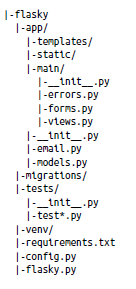
\includegraphics[scale=0.75]{figs/FlaskProjectStructure.png}
    \caption{Structura unui proiect Python utilizand Flask \cite{flaskweb}}
    \label{fig:FlaskProjectStructure}
\end{figure}

Structura de proiect prezentata in figura \ref{fig:FlaskProjectStructure} este detaliata in cele ce urmeaza:
\begin{enumerate}
	\item Fisierul flasky.py contine apelul prin care obiectul Flask este pornit, metoda run(). Aceasta metoda primeste ca parametrii adresa si 
    portul prin care serverul poate fi accesat. Este punctul principal, sau punctul de intrare in aplicatie si reprezinta o bucla infinita 
    in care sunt deservite cererile de la client.
	\item Fisierul requirements.txt contine numele bibliotecilor utilizate in proiect si versiunile acestora. Este un fisier foarte util atunci 
	cand o persoana preia proiectul pe o masina diferita si are nevoie sa creeze un mediu de lucru. Continutul acestui fisier poate fi usor generat 
    de comanda "pip freeze".
    \item Directorul venv/ contine toate bibliotecile instalate, cele continute in fisierul requirements.txt, si o referinta catre versiunea de python 
    utilizata. Astfel se creeaza un mediu de lucru separat fata de ceea ce este instalat global pe computer sau de alte proiecte. Acest director 
    trebuie creeat in faza de initiere a proiectului si atunci cand este preluat pe o alta masina de lucru.
    \item Directorul app contine fisierele aplicatiei, toate fisierele necesare ca aplicatia sa ruleze. Directoarele pentru testare si migrari sunt 
    separate.
    \item Fisierul view.py contine partea de rutare a cerintelor primite de la client catre resurse prin decoratori sau prin metode statice si 
    partea de formatare a raspunsului in structura asteptata de client. Acest fisier poate fi impartit in doua modula separate, routes.py si 
    view.py, fiecare avand o sarcina bine definita.
    \item Fisierul \_\_init\_\_.py din directorul app contine instantierea clasei Flask. Acest obiect se ocupa de toate cererile care vin de la client. 
    Pe langa instantiere mai poate contine metode de initializare a diferite module sau biblioteci pe care aplicatia le utilizeaza, cum ar fi conexiunea 
    la baza de date sau un sistem de versionare. Orice director care contine acest fisier este considerat un packet reutilizabil care poate fi inclus si 
    utilizat intr-o alta aplicatie. Atunci can directorul app este inclus in aplicatie, continutul fisierului \_\_init\_\_.py este prima portine de 
    cod care se ruleaza din acel pachet. 
\end{enumerate}

Decoratorii in python reprezinta o metoda prin care se seteaza o portiune de cod care sa fie executata atunci cand anumite evenimente au loc. De exemplu, 
la primirea unei cereri de la client decoratorul spune care portiune de cod, metoda, trebuie executata. In general aceasta metoda poarta denumirea de 
Handler. Decoratorii de tip route fac legatura intre adresa URL primita de la client si metodele resursei indentificata unic de adresa URL. Modul in  
care aceasta legatura este realizata de Flask, este prin creearea unei mapari a adreselor URL pe resurse.

Argumentele dinamice in adresa URL sunt adrese URL de baza care identifica o resursa, dar care au in plus un argument ce poate lua orice valoare. Acest 
argument este preluat de catre resursa si pe baza lui raspunsul care s-ar fi trimis in mod normal este personalizat generand un raspuns diferit.

Flask ofera un serviciu numit Request Hooks care ofera posibilitatea de a executa portiuni de cod inainte ca fiecare cerere de la client sa fie procesata, 
inainte doar de prima cerere de la client sau dupa ce cererea a fost procesata. Acest serviciu este util pentru cazurile in care se doreste realizarea 
conexiunii la baza de date sau autentificarea clientului de fiecare data cand o cerere este receptionata. Avantajul utilizarii acestui serviciu este 
cantitatea redusa de cod duplicat. Il loc sa se realizeze autentificarea in fiecare rutina specifica unei resurse, se realizeaza in mod generic inainte ca 
resursa sa fie accesata.

Cazurile de eroare, in Flask, pot fi personalizate. La primirea unei cereri de la client, daca aceasta este eronata, se poate transmite ca raspuns, pe langa 
codul de eroare, o pagina HTML sau un text care sa explice de ce a fost respinsa cererea.

Unele framework-uri din Python contin setul de instructiuni pentru integrara cu Flask, dar, dupa cum am prezentat si mai sus, Flask a fost creat pentru a fi 
integrat cu module externe, deci instructiunile necesare pentru integrarea cu acesta pot fi scrise de utilizator. Un exemplu de framework pentru baze de date 
care este integrat cu Flask este Flask-SQLAlchemy.

Micro-framework-ul Flask are un grad de flexibilitate foarte inalt comparat cu un full-framework. Flask a fost creat pentru a automatiza doar functionalitatile 
de baza necesare unei apicatii web, ceea ce inseamna ca nu are integrate componente pentru autentificare sau operatii pe baze de date, dar este 
compatibil cu componente externe. Acest lucru ofera posibilitatea de a utiliza framework-ul impreuna cu orice fel de baza de date sau orice tip de 
autentificare. Pe cealalta parte, un framework full, ca Django, ofera o gama de componente care pot fi utilizate pentru functionalitati precum 
operatiile pe baze de date si autentificare, deci utilizatorul este restrans in ceea ce priveste functionalitatile proiectului lui.

\subsection{Retrofit framework}\label{sec:retrofit}
Retrofit este o biblioteca scrisa in limbajul de programare Java care are scopul de a simplifica tranzactionarea cu un server RESTful. Intr-o arhitetura 
client-server aceasta biblioteca este implementata in partea clientului si este o interfata API care respecta constrangerile arhitecturii REST. Este o 
biblioteca utilizata cu preponderenta in aplicatiile pentru sistemul de operare Android. In urmatoarele paragrafe sunt descrise caracteristicile cheie 
ale acestei biblioteci.

Aceasta biblioteca nu are implementat propriul mechanism petru tranzactionarea pachetelor HTTP, ci este integrata cu biblioteca OkHTTP. Aceasta din 
urma este o biblioteca complexa care implementeaza protocolul HTTP si toate mecanismele necesare de mitigare si rezolvare a erorilor in tranzactionarea 
prin retea. Are scopul de a automatiza complexitatea tranzactionarii prin retea pentru a usura utilizatorul de aceasta sarcina.
 
Biblioteca Retrofit este construita peste OkHTTP si rolul ei este de a automatiza parsarea si formatarea cererilor si raspunsurilor HTTP. Aceasta creeaza 
adresa URL si o trimite bibliotecii OkHTTP de unde este trimisa in retea. La primirea raspunsului, OkHTTP il trimite catre Retrofit care se ocupa de formatarea 
lui pentru a-l prezenta utilizatorului sub structura dorita, de exemplu, un obiect.

Figura \ref{fig:RetrofitStructure} prezinta functionalitatea bibliotecii retrofit. Aceasta va fi detaliata in paragrafele urmatoare.
\begin{figure}[H]
    \centering
    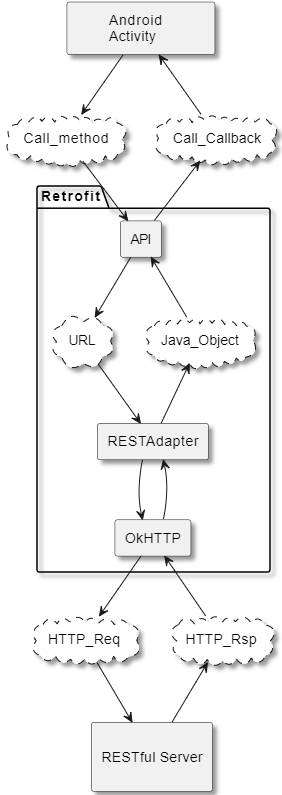
\includegraphics[scale=0.55]{figs/RetrofitStructure.png}
    \caption{Structura bibliotecii Retrofit}
    \label{fig:RetrofitStructure}
\end{figure}

Modulul Android Activity reprezinta interfata cu utilizatorul in sistemul de operare android. In urma unui eveniment, de exemplu, apasare buton sau 
o rutina periodica, se trimite o cerere catre modulul API, care la finalul tranzactiei va returna informatia care va fi afisata utilizatorului.

Modulul API contine mai multe modele si o interfata. In interfata sunt declarate metodele utilizate pentru a obine date de la server, de exemplu, metoda 
GetAllClients care va informa serverul sa puna in raspuns o lista cu toti clientii din baza de date. Utilizand adnotari aceste metode sunt mapate pe adrese URL. 
Metode returneaza un model, acesta fiind o clasa care contine toate campurile primite de la server in raspuns. De exemplu, campurile nume, adresa, 
varsta. La construirea obiectului Retrofit se realizeaza maparea dintre adresa URL, metode, si modele. API trimite catre modulul RESTAdapter un obiect 
al clasei Call. Acest obiect este initializat cu metoda care se doreste a fi executata utilizand obiectul Retrofit. Acesteia i se mai ataseaza 
doua rutine, una care este executata in cazul in care tranzactia a fost efectuata cu success si una care se executa in caz 
contrar.

Modulul RESTAdapter primeste de la modulul API obiectul de tip Call care contine toate informatiile necesare pentru a executa cererea catre server. Obiectul Call 
este transpus in format OkHTPP si trimis catre modulul OkHTTP. La finalul tranzactiei acesta primeste un raspuns de tipul OkHTTP pe care il mapeaza, 
pe baza informatiilor din obiectul retrofit, intr-un obiect al clasei model specifice. Acest obiect este returnat modulului API.

Modulul OkHTTP se ocupa de tranzactionarea efectiva prin retea. Primeste si returneaza obiecte specifice acestei biblioteci.

Fiecare metoda din Retrofit este identifica unic de o adresa URL si identifica unic un set de date cerut de la un server. Fiecare set de date este 
reprezentat printr-o clasa model. Acest lucru face posibila maparea dintre URL, metoda si model. Metodele sunt mapate la adrese URL prin adnotari. 
In aceste adnotari se specifica metoda HTTP si adresa URL. Cele mai utilizate adnotari sunt prezentate mai jos:
\begin{enumerate}
	\item @Path - aceasta adnotare permite utilizarea de campuri variabile in adresa URL. Aceasta adnotare este un parametru al functiei, iar valoarea 
	pe care o primeste la apelul metodei este pusa in adresa URL.
    \item @Body - aceasta adnotare permite inserarea in adresa URL a unei clase model. Aceasta adnotare se utilizeaza la metodele HTTP de salvare 
    in baza de date, cum ar fi metoda POST.
    \item @FormUrlEncoded - aceasta adnotare permite inserarea in adresa URL a unor campuri dintr-un model cu scopul de a-l modifica in baza de date.
\end{enumerate}

Metodele in Retrofit sunt doar declarate intr-o interfata, nu si implementate, iar instructiunile necesare pentru a converti o cerere HTTP intr-o clasa java 
sunt generate automat de catre acesta. Retrofit suporta conversia automata a multor tipuri de format a datelor, cum ar fi GSON sau SimpleXML, dar acopera si 
cazul in care serverul returneaza un format de date care nu este suportat, prin crearea unui convertor particular. Acest lucru presupune scrierea 
manuala a instructiunilor necesare convertirii raspunsului de la server in obiect Java. Acest lucru nu trebuie facut petru fiecare resursa in parte, ci 
in mod general, o singura data.

GSON este o biblioteca in Java care are rolul de a serializa un obiect Java intr-un format JSON, respectiv de a deserializa un obbiect in format JSON intr-un 
obiect java.   

Clasa Call suporta executarea cererii HTTP in mod sincron sau asincron. Este de preferat modul asincron, deoarece executia are loc pe un fir separat lasand 
firu de executie creator sa execute alte sarcini. Aceasta clasa este dedicata pentru fiecare tranzactie, o instanta a acesteia poate fi utilizata pentru 
o singura transmisie a unei cereri HTTP si receptie a unui raspuns HTTP. La finalul unei tranzactii obiectul este distrus.

\section{Baza de date MongoDB}\label{sec:mongodb}
MongoDB este o baza de date orientata pe documente fiind printre putinele baze de date diferita de cele uzuale care sunt relationale, adica stocheaza datele in tabele 
grupate intre ele prin relatii. Aceasta baza de date stocheaza datele in colectii de documente, de aici si denumirea de baza de date orientata pe documente. 
Structura acestui tip de baze de date permite un grad inalt de scalabilitate prin impartirea si distribuirea unei baze de date foarte mari pe mai multe 
servere. In paragrafele care urmeaza vor fi descrise caracteristicile cheie ale bazei de date.

Documentul reprezinta un singur set de date si poate fi asociat cu un inlocuitor al unui rand dintr-o baza de date relationala. Setul de date este stocat intr-un 
format numit BSON, Binary-JSON, care este o reprezentare in binar a formatului de fisiere JSON. Acesta din urma este un format de fisiere bazat pe text,
are o structura de tipul cheie-valoare si este usor de interpretat de catre om.

Figura \ref{fig:MongoDBDocument} prezinta structura unui document dintr-o baza de date MongoDB si, de asementea, formatul JSON.
\begin{figure}[H]
    \centering
    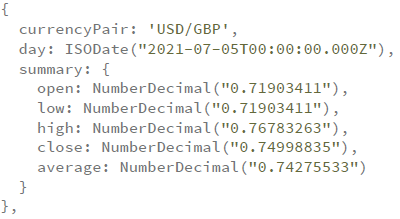
\includegraphics[scale=0.8]{figs/mongoDBDocument.png}
    \caption{Exemplu de document \cite{mongoDB}}
    \label{fig:MongoDBDocument}
\end{figure}

Colectiile de tip serii in timp reprezinta un tip de colectii optimizate pentru a stoca si interoga documentele ordonate in timp. Aceste documente au in 
componenta un camp obligatoriu care reprezinta momentul de timp la care datele au fost achizitionate. In documentul prezentat in figura \ref{fig:MongoDBDocument} 
se poate observa perechea de valori "day" si data si ora in format ISO. Acest tip de colectii este utilizat cu preponderenta in IoT datorita faptului ca sunt 
optimizate pentru structura de date uzuala unui senzor. O astfel de structura contine, in general, un moment de timp la care achizitia de date a fost efectuata, 
un identificator unic al senzorului, in mod uzual adresa MAC, si valoarea metricii sau a metricilor achizitionate.

MongoDB creeaza automat un indice, o cheie primara, pentru fiecare document pentru a se asigura ca nu exista doua documente cu acelasi indice. In acelasi timp 
permite creearea unui indice secundar care poate contine unul sau mai multe campuri din setul de date si care are ca scop plierea pe structura fiecarui set de date 
si pe tipul de interogari cel mai des efectuate. In cazul seriilor in timp cele mai uzuale interogari sunt bazate pe timp, deci indicele ar trebui sa contina campul 
de timp la care trebuie specificata si ordonarea elementelor, de exemplu, intr-un sistem in care interogarea cea mai des intalnita este retragerea documentelor 
din ultimele 24 de ore ordonarea trebuie efectuata in ordine descrescatoare a timpului. Pe langa campul de timp, indicele mai poate contine inca un camp pentru 
a acoperi cazurile in care interogarea se face nu doar pe o perioada de timp, ci si pe o alta valoare continuta in setul de date, de exemplu, campul care contine 
adresa MAC a senzorului. MongoDB va stoca datele in functie de acest indice obtinand astfel interogari foarte eficiente. Totodata un indice prea complex sau 
scris incorect va creste complexitatea scrierii in baza de date si automat va scadea eficienta.
